\Aufgabe{BYCS Drive}{%
    \begin{minipage}[t]{0.5\textwidth}
        \vspace{0pt}
        \begin{enumerate}
            \item Öffne \UrlAndCode{drive.bycs.de} im Internetbrowser und melde dich mit deinen BYCS/Mebis Logindaten an. \\
                \hinweis{Internetbrwoser zeigen Websites an und sind unser üblicher Zugang zum Internet. Bekannte Browser sind \textbf{Mozilla Firefox}, Google Chrome oder Microsoft Edge.}
            \item Erstelle einen in deinem persönlichen Bereich einen neuen Ordner mit Name \emph{Informatik\_09}
            \item Wenn du in diesem Ordner auf \emph{+Neu} klickst kannst du neue Dateien (z.B. Kalkulationstabellen) erstellen.\\
                \emphColB{WICHTIG:} Achte darauf, die Dateiendung (nach dem Punkt, z.B. \emphColB{.xlsx}), nicht zu verändern!
        \end{enumerate}
    \end{minipage}
    \hfill
    \begin{minipage}[t]{0.45\textwidth}
        \ifbeamer
            \vspace{3.5cm}
        \else
            \vspace{0pt}
        \fi
        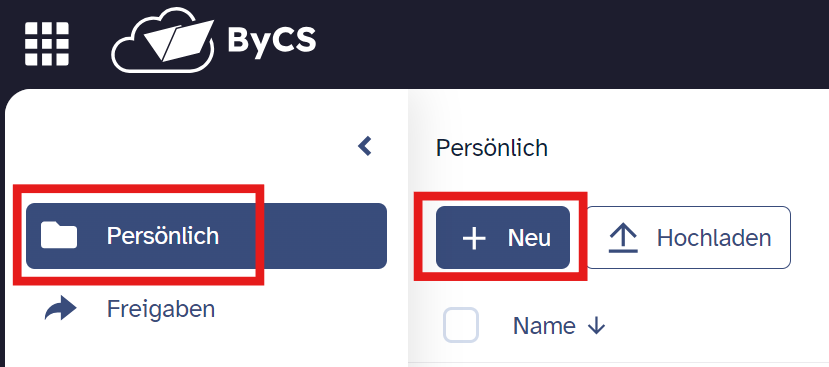
\includegraphics[width=\textwidth]{Aufgaben/TabKalk_DFD/img/A00_newFolder.png}
    \end{minipage}
}
